\documentclass[11pt,a4paper]{article}
\usepackage[margin=2.5cm]{geometry}
\usepackage[T1]{fontenc}
\usepackage[utf8]{inputenc}
\usepackage{lmodern}
\usepackage{graphicx,booktabs,siunitx,xcolor,amsmath}
\usepackage[hidelinks]{hyperref}
\usepackage{caption}
\sisetup{group-separator={,},range-phrase={ to }}
\newcommand{\gapbs}{GAPBS}

\title{Performance Engineering\\Project: Breadth-First Search in GAPBS}
\author{Group1\\Sergiu Alexandru Macra s5524032\\Cosmin Andrei Stamate s5600723}
\date{October 2026}

\begin{document}
\maketitle

\begin{abstract}
\noindent We looked at the breadth-first search (BFS) kernel of the GAP Benchmark Suite on
two systems: our laptop (Intel Core i7-12650H, under WSL2) and one node of the Hábrók
cluster (two AMD EPYC 7763). We measured it with perf, PAPI, gprof, the timers of the
benchmark and a small counter tool we wrote ourselves, and we checked these tools against
each other. Most of the time goes to the bottom-up step and to threads waiting at OpenMP
barriers. By counting the work, we found that a search only looks at \SI{4.7}{\percent} of
the edges of the graph. Our model, based on this count and on the measured bandwidth,
latency and memory-level parallelism, shows that one thread is limited by memory latency,
the laptop with all threads by memory bandwidth, and the Hábrók node by synchronisation and
the two sockets. We tried seven optimisations. Three of them gave a clear improvement:
relabelling the vertices by degree (2.4 times faster on the laptop, 1.8 times on Hábrók for
a larger graph), using fewer threads on one socket (2.1 times) and spreading the graph over
both NUMA nodes (2.1 times when the threads are spread). Compiler flags, schedules, huge pages and prefetching stayed within the noise.
\end{abstract}

\section{Introduction}

Breadth-first search (BFS) is the typical example of the graph traversal dwarf. It is the
main kernel of Graph500~\cite{graph500} and one of the six kernels of the GAP Benchmark Suite
(\gapbs)~\cite{beamer2015gap}. BFS does almost no arithmetic. Its speed depends on how fast
it can get data from memory, and most of these accesses are random. Because of this, a
model of BFS has to describe data movement, latency and synchronisation, and not
floating-point operations.

The goal of the project was not to write the fastest BFS, but to go through the full
performance engineering process with the \gapbs{} reference code:
\begin{enumerate}
  \item analyse the program with more than one tool, and check that the tools give correct
        results,
  \item explain the measurements with a model whose parameters we measured ourselves,
  \item choose, implement and test optimisations based on the analysis and the model.
\end{enumerate}

In our work plan we wanted to use a laptop and the HAICGU cluster. We did not get access to
HAICGU, so we used the Hábrók cluster of the university instead. We also did more
memory and OpenMP optimisations than planned, because the analysis showed that these parts
take most of the time, and fewer compiler optimisations.

% Owner: Sergiu
\section{Application: direction-optimising BFS in \gapbs}
\label{sec:app}

\gapbs{} stores graphs in compressed sparse row (CSR) form: an index array of $n{+}1$ 8-byte
pointers and a neighbour array of 4-byte vertex IDs. An undirected graph stores every edge in
both directions. Our main input is a Kronecker graph with scale 20 (\texttt{kron20}:
$n = 2^{20}$ vertices, $m = \num{15699691}$ undirected edges, \SI{136}{MB} in memory). It is
generated once and loaded from a serialised file, because generating and building the graph
took \SI{84}{\percent} of a naive benchmark run. Larger graphs (\texttt{kron22},
\texttt{kron24}: \SIlist{0.5;2.1}{GB}) are used to vary the working set.

The kernel (\texttt{src/bfs.cc}) implements direction-optimising BFS~\cite{beamer2012do}. It
returns the BFS parent of every vertex and uses five performance-relevant routines:
\begin{description}
  \item[\texttt{TDStep}] (top-down): every vertex in the frontier queue scans its neighbours and
        claims unvisited ones with an atomic compare-and-swap on \texttt{parent[v]}. The access to
        \texttt{parent[v]} is random. Parallelised over the queue (static schedule).
  \item[\texttt{BUStep}] (bottom-up): every \emph{unvisited} vertex scans its neighbours until
        it finds one in the frontier bitmap, then stops (early exit). It sweeps all $n$
        vertices; neighbour lists are read from their start. Parallelised with
        \texttt{schedule(dynamic,1024)}.
  \item[\texttt{QueueToBitmap}, \texttt{BitmapToQueue}] convert the frontier when the
        direction changes.
  \item[\texttt{InitParent}] initialises \texttt{parent} with negated degrees once per search.
\end{description}
\texttt{DOBFS} switches to bottom-up when the edges leaving the frontier exceed
$1/\alpha$ of the unexplored edges, and back when the frontier shrinks below $n/\beta$
(defaults $\alpha{=}15$, $\beta{=}18$).

\paragraph{Work actually performed.} We added an optional edge counter
(\texttt{-DPE\_COUNT\_EDGES}). Averaged over 16 searches on \texttt{kron20}, a search performs
4.25 top-down and 2.5 bottom-up steps and examines \num{286935} edges top-down and
\num{1202922} edges bottom-up. That is only \SI{4.7}{\percent} of the \num{31399382}
directed edges. Bottom-up checks \num{1659885} vertices in total, most of which find a parent
in the frontier after reading fewer than one cache line of neighbours. Throughput is
conventionally reported in traversed edges per second (TEPS), counting all $m$ input edges
(we follow this convention). TEPS therefore overstates the edges actually touched by about
$20\times$, and a model must be based on the real work (Section~\ref{sec:model}).

\section{Systems and environment}
\label{sec:systems}

\begin{table}[ht]
\centering\footnotesize
\caption{The two systems. Bandwidth and latency were measured by us (Section~\ref{sec:model}).}
\label{tab:systems}
\begin{tabular}{@{}p{3.3cm}p{5.7cm}p{5.4cm}@{}}
\toprule
 & Laptop & Hábrók node (\texttt{regular}) \\
\midrule
CPU & Intel Core i7-12650H & 2 $\times$ AMD EPYC 7763 (Zen 3) \\
Cores & 6 P-cores + 4 E-cores (16 threads), WSL2 shows 10 vCPUs & 2 $\times$ 64 cores, no SMT, 2 NUMA nodes \\
Caches & L1d \SI{48}{KiB} per core, L3 \SI{24}{MiB} & L2 \SI{512}{KiB} per core, L3 16 $\times$ \SI{32}{MiB} (one per CCD) \\
Memory & one DDR4-3200 channel (\SI{25.6}{GB/s} peak), \SI{7.6}{GiB} visible in WSL2 & \SI{503}{GiB} \\
STREAM triad, all / 1 thread & \SI{15.9}{GB/s} / \SI{12.3}{GB/s} & \SI{327}{GB/s} / \SI{34.7}{GB/s} \\
Load latency at \SI{1}{GB} & \SI{376}{ns} & \SI{99}{ns} \\
OS & Ubuntu 24.04.1 on WSL2, Linux 6.18 & AlmaLinux 9.8 \\
Compiler & GCC 13.3, \texttt{-O3 -fopenmp} & GCC 11.5, \texttt{-O3 -fopenmp} \\
Transparent huge pages & \texttt{madvise} (default) & \texttt{always} \\
Tools & perf 6.18 (software events and sampling), gprof & PAPI 7.1 (built by us), pecount, gprof \\
\bottomrule
\end{tabular}
\end{table}

Table~\ref{tab:systems} shows the two systems. All builds also use \texttt{-g
-fno-omit-frame-pointer}, so that perf can record call graphs. This does not change the code
of the loops.

\paragraph{Laptop under WSL2.} WSL2 runs Linux in a Hyper-V virtual machine, and this limits
what we can measure on the laptop:
\begin{itemize}
  \item The hardware counters are not passed through to the virtual machine. All hardware
        events (cycles, instructions, cache and TLB misses) give \emph{not supported}. Only
        software events and timer-based sampling work.
  \item The virtual machine shows 10 vCPUs and does not tell which ones are P-cores and
        which are E-cores, so we cannot choose between them.
  \item The memory addresses are translated twice (nested paging). This is probably one
        reason for the high memory latency of \SI{376}{ns}, and it also adds noise.
\end{itemize}
The laptop has only one memory channel with a peak of \SI{25.6}{GB/s}. STREAM reaches
\SI{15.9}{GB/s} with all threads, which is \SI{62}{\percent} of the peak. In Assignment 6 we
saw on the same laptop that STREAM is fastest with about four threads and gets slower with
more threads. We wanted to boot a native Linux on the laptop to get hardware counters, but we
did not manage this in time, so all hardware counters come from Hábrók.

\paragraph{Hábrók.} The compute nodes have no \texttt{perf}, no \texttt{numactl} and no PAPI
module, and \texttt{perf\_event\_paranoid} is set to 2, so we can only count events in user
space. We therefore built PAPI 7.1 from source in our home directory. We also wrote
\texttt{pecount} (\texttt{pe/bench/pecount.c}, about 200 lines), which counts the events of a
program with \texttt{perf\_event\_open}, like \texttt{perf stat} does. All Hábrók runs used one
full node (exclusive) through Slurm. Still, when several counters were open, they were only
active \SIrange{14}{26}{\percent} of the time. Probably other software on the node also uses
the counters. For exact counts we therefore use PAPI regions with only a few events.

\section{Measurement method and checking the tools}
\label{sec:method}

\paragraph{Changes to the code.} All our changes are compile-time switches in
\texttt{src/pe\_opts.h}. Without them the code behaves like the original \gapbs. The only
change in the default build is that every \texttt{\#pragma omp parallel for} is split into
\texttt{parallel} and \texttt{for}, which does the same thing. With the switches we can turn on
PAPI regions inside every parallel region (the PAPI high-level API only counts the thread
that calls it), the edge counter, \texttt{schedule(runtime)}, prefetching, huge pages,
parallel first touch, relabelling and other values of $\alpha$ and $\beta$. A script builds 27
variants, and every variant has to pass the BFS verifier of \gapbs{} (\texttt{-v}) before we
time it.

\paragraph{How we time.} For every configuration we first do one run that we throw away, and
then 5 runs of 24 searches each. The sources of the searches are chosen pseudo-randomly, but
they are the same for all variants and both machines. We use the timer of \gapbs{} around
one search. Inside one run the first searches are slow (Figure~\ref{fig:warmup}): on Hábrók
the first five take between 99 and \SI{156}{ms}, and after that about \SI{4}{ms}. So we drop
searches 1 to 5 of every run, which leaves 95 samples per configuration. As in the lectures,
we report the median and the interquartile range (IQR) in ms per search, and GTEPS $=
m/t_\text{median}$. The IQR is between \SI{14}{\percent} (Hábrók, kron22) and
\SI{56}{\percent} (laptop, kron20) of the median. We only call a difference significant if it
is bigger than the IQR of both configurations.

\begin{figure}[ht]
\centering
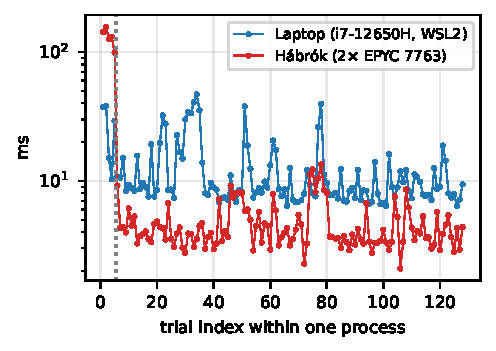
\includegraphics[width=0.55\linewidth]{figures/warmup.pdf}
\caption{Time of every search inside one run (128 searches, log scale). The slow first
searches on Hábrók and the outliers on the laptop are the reason why we drop searches 1 to 5
and use the median.}
\label{fig:warmup}
\end{figure}

\paragraph{Checking the tools.} Before we use a tool, we want to know that it measures the
right thing. Table~\ref{tab:validation} shows our checks.
\begin{table}[ht]
\centering\small
\caption{Checks of the measurement tools.}
\label{tab:validation}
\begin{tabular}{@{}p{3.4cm}p{6.1cm}p{4.6cm}@{}}
\toprule
Check & Result & Conclusion \\
\midrule
Timer resolution & \texttt{CLOCK\_MONOTONIC}: \SI{1}{ns}, one call takes \SIrange{34}{36}{ns} & small compared to a search (more than \SI{1}{ms}) \\
Wall time from 3 tools (laptop, 64 searches) & \gapbs{} load + searches \SI{0.679}{s}, perf \texttt{duration\_time} \SI{0.717}{s}, \texttt{/usr/bin/time} \SI{0.69}{s} & they agree, the \SI{38}{ms} difference is starting the program \\
CPU time from 2 tools & perf task-clock \SI{6.00}{s}, \texttt{time} user + sys \SI{6.05}{s} & within \SI{1}{\percent} \\
pecount against perf & page faults \num{36422} and \num{36423} & pecount gives the same result \\
gprof & \SI{100}{\percent} of the samples in \texttt{frame\_dummy} & \textbf{not usable} for OpenMP: it does not assign the time of the OpenMP threads to the right functions \\
perf sampling & BUStep, InitParent and TDStep are found; libgomp has no symbols but is found by library & reliable \\
PAPI against pecount (Hábrók, 1 thread, 64 searches) & sum of the 5 PAPI regions divided by pecount: cache misses \SI{99.1}{\percent}, references \SI{97.2}{\percent}, cycles \SI{95.0}{\percent}, instructions \SI{90.3}{\percent} & they agree, the rest is code outside the regions (last loop, bitmap resets) \\
Known result: integer loop (PAPI) & \num{5.000} instructions and \num{4.000} cycles per iteration & the loop has 5 instructions, \texttt{imul} (3 cycles) + \texttt{add} (1 cycle) \\
Known result: pointer chase over \SI{1}{GB} (PAPI) & \num{1.0007} cache misses per step & one miss per random load, as expected \\
Known results with pecount & loop: \num{4.99} instructions per iteration; chase: \num{2.4} misses per step & counters were shared (multiplexed), and the scaling is wrong when the program has phases, so we use PAPI regions \\
Timers on Hábrók & \texttt{/usr/bin/time} is not installed & cross-check only on the laptop \\
\bottomrule
\end{tabular}
\end{table}

\paragraph{The verifier found a data race.} Running the verifier on every variant was useful.
With \texttt{schedule(runtime)} and \texttt{OMP\_SCHEDULE=dynamic,100} or \texttt{guided},
\emph{every} search gave a wrong BFS tree (0 of 8 correct on both machines), and
\texttt{static,1000} was wrong in 4 of 8 searches on the laptop and in all 8 on Hábrók. The
reason is that \texttt{BUStep} sets bits in the shared \texttt{next} bitmap with a normal,
non-atomic read-modify-write of a 64-bit word. This is only safe when the block of every
thread starts at a word boundary, so when the chunk size is a multiple of 64. The original
\texttt{dynamic,1024} fulfils this without saying so. Plain \texttt{static} passed our tests,
but only by luck, because its blocks also do not have to start at a word boundary. In the
schedule experiments we therefore only used chunk sizes that are a multiple of 64.

% Owners: Cosmin (laptop), Sergiu (Hábrók counters)
\section{Performance analysis}
\label{sec:analysis}

\paragraph{Baseline.} On \texttt{kron20}, the original \gapbs{} with the default number of
threads needs \SI{8.58}{ms} per search on the laptop (median, IQR \SI{4.77}{ms},
\SI{1.83}{GTEPS}) and \SI{2.85}{ms} on Hábrók (IQR \SI{1.43}{ms}, \SI{5.51}{GTEPS}). The Hábrók
node has 12.8 times more cores and 20 times more memory bandwidth, but it is only 3 times
faster. The main question of our analysis is why.

\paragraph{Hotspots.} Table~\ref{tab:hotspots} shows where the laptop spends its time,
measured with perf sampling (about \num{46000} samples, 64 searches, all threads).
\begin{table}[ht]
\centering\small
\caption{Laptop, perf sampling (task-clock, \SI{5}{kHz}), \texttt{kron20}, 64 searches including loading the graph.}
\label{tab:hotspots}
\begin{tabular}{@{}lrl@{}}
\toprule
Function & Samples & What it does \\
\midrule
OpenMP runtime (\texttt{libgomp}) & \SI{50.0}{\percent} & threads waiting at barriers \\
\texttt{BUStep} & \SI{35.8}{\percent} & bottom-up step \\
\texttt{InitParent} & \SI{5.7}{\percent} & initialisation of every search \\
\texttt{TDStep} & \SI{3.1}{\percent} & top-down step \\
\texttt{BitmapToQueue} + \texttt{QueueToBitmap} & \SI{2.4}{\percent} & frontier conversion \\
\texttt{DOBFS} (last loop) and rest & \SI{3.0}{\percent} & \\
\bottomrule
\end{tabular}
\end{table}
Half of all CPU time is spent by threads that wait in the OpenMP runtime. One search has
about ten short parallel regions (Section~\ref{sec:app}) and each of them ends with a barrier.
The work inside them is not balanced: Kronecker graphs have a few vertices with a very high
degree, and in bottom-up the cost of a vertex depends on how fast it finds a neighbour in
the frontier. Of the useful work, \texttt{BUStep} is by far the biggest part. With
\texttt{perf annotate} (\texttt{pe/results/wsl/perf\_annotate\_all.txt}) we looked at the
instructions of \texttt{BUStep}. \SI{39}{\percent} of its samples are on the instruction just
after the load of the first neighbour ID. With timer sampling, the sample usually lands on
the instruction that uses the result of a slow load, so this is the cache miss at the start
of every neighbour list. Another \SI{11}{\percent} are on the bit test of the bitmap and about
\SI{13}{\percent} on loads of the CSR index. So the time is spent on memory accesses, not on
computation.

\paragraph{Hardware counters per function (Hábrók).} With PAPI regions we can measure every
function separately, which sampling on the laptop cannot do (Table~\ref{tab:papi}). We used one
thread, so that every region is fully counted.
\begin{table}[ht]
\centering\small
\caption{PAPI per function, Hábrók, 1 thread, \texttt{kron20}, per search (64 searches).
Misses are the generic event \texttt{PERF\_COUNT\_HW\_CACHE\_MISSES}.}
\label{tab:papi}
\begin{tabular}{@{}lrrrrr@{}}
\toprule
Function & Cycles [M] & Share & IPC & Cache misses [k] & Misses per unit of work \\
\midrule
\texttt{BUStep} & 64.0 & \SI{77.7}{\percent} & 0.77 & 532 & 0.32 per checked vertex \\
\texttt{InitParent} & 11.6 & \SI{14.0}{\percent} & 0.89 & 3.7 & - \\
\texttt{TDStep} & 3.6 & \SI{4.4}{\percent} & 1.01 & 216 & 0.75 per examined edge \\
\texttt{BitmapToQueue} & 2.4 & \SI{2.9}{\percent} & 4.80 & 0.2 & - \\
\texttt{QueueToBitmap} & 0.8 & \SI{0.9}{\percent} & 1.59 & 2.5 & - \\
\bottomrule
\end{tabular}
\end{table}
Even without any synchronisation, \texttt{BUStep} takes \SI{78}{\percent} of the cycles. Both
steps run at an IPC of about 1, while the core could do several instructions per cycle. In
\texttt{TDStep}, \SI{75}{\percent} of the examined edges give a cache miss, which is what we
expect for the random accesses to \texttt{parent[v]}. In \texttt{BUStep} only a third of the
checked vertices give a miss. The neighbour lists of vertices that follow each other are next
to each other in the CSR array, so the hardware prefetcher can load many of them in time. The
two conversion functions are simple bit operations with a high IPC, and they cost very little.

Branches also cost time. With one thread a search has 17.8 million branches, and 2.3 million
of them are mispredicted (\SI{12.9}{\percent}, measured with pecount). Most of them come from
the bit test and the early exit in \texttt{BUStep}, which depend on the data. A misprediction
typically costs 10 to 20 cycles, so this can be a large part of the 87 million cycles of a
search, although part of it overlaps with the waiting for memory.

The data TLB is not a problem on Hábrók: transparent huge pages are always on there, and one
search only has about \num{4200} dTLB misses, compared to about 2 million random accesses. We
also measured the counters with 128 threads, but these runs include the five slow first
searches, which take most of the run time, so we do not use these numbers.

\paragraph{Scaling with the number of threads.} Figure~\ref{fig:scaling} shows the time per
search for different numbers of threads. On the laptop the best time is with 8 threads
(\SI{8.39}{ms}). With 10 threads it is not faster, and the IQR becomes much larger
(\SI{12.3}{ms}). On Hábrók the time goes down until 48 to 64 threads that are bound to
neighbouring cores (\SI{1.38}{ms}, \SI{11.4}{GTEPS}), and then it goes \emph{up} again, to
\SI{3.53}{ms} with 128 threads. With \texttt{OMP\_PROC\_BIND=close}, 64 threads fill exactly
one socket. When the second socket is used, \texttt{parent} and the bitmaps have to be kept
coherent between the two sockets, more threads have to meet at every barrier, and every
thread has less work. Without binding, the best time is \SI{2.45}{ms} with 48 threads.

\begin{figure}[ht]
\centering
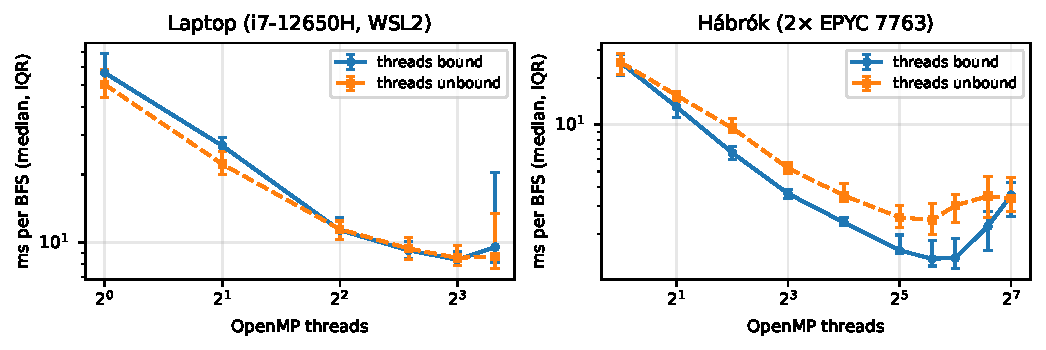
\includegraphics[width=\linewidth]{figures/scaling.pdf}
\caption{Time per search on \texttt{kron20} against the number of OpenMP threads, with the
threads bound to neighbouring cores (\texttt{OMP\_PROC\_BIND=close},
\texttt{OMP\_PLACES=cores}) and not bound (median, error bars: IQR).}
\label{fig:scaling}
\end{figure}

\paragraph{Memory hierarchy.} Figure~\ref{fig:latency} shows the latency of dependent loads on
both machines, measured with a pointer chase over a random cycle. The steps show the cache
sizes. On Hábrók the latency stays at 13 to \SI{15}{ns} up to \SI{32}{MiB} (the L3 of one
CCD) and is about \SI{99}{ns} in main memory. On the laptop it goes up to \SI{376}{ns} at
\SI{1}{GB}, probably because of TLB misses with nested paging. The working set of one
\texttt{kron20} search is about \SI{180}{MB} (Section~\ref{sec:model}). This is bigger than
all caches of the laptop. On Hábrók it is bigger than the L3 of one CCD, but would fit in all
16 L3 slices together. A core can only use the L3 of its own CCD, so data cached by another
CCD probably has to come over the interconnect, with a latency close to main memory.

\begin{figure}[ht]
\centering
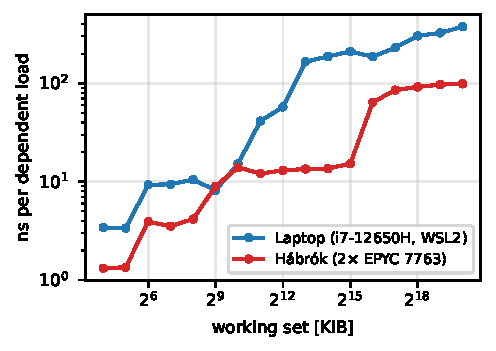
\includegraphics[width=0.55\linewidth]{figures/latency.pdf}
\caption{Latency of dependent loads against the size of the working set (one core).}
\label{fig:latency}
\end{figure}

% Owner: Sergiu
\section{Performance model}
\label{sec:model}

\paragraph{Which model.} BFS does almost no floating-point operations, so a normal roofline
in FLOP/byte~\cite{roofline} does not make sense here. If we use examined edges as the unit of
work instead, the arithmetic intensity is only 1.49 million edges per \SI{179}{MB}, so about
\num{0.008} edges per byte. The ECM model needs a loop that always does the same work with
predictable data transfers, so that in-core time and transfer time can be added. BFS has early
exits that depend on the data, atomic operations, and the work changes in every level, so
ECM does not fit either. We therefore used the information exchange model from the lectures:
we count how many bytes have to be moved and how many random accesses have to be waited
for, based on the work we counted and not on the size of the graph. Then we compute two
lower bounds, one for bandwidth and one for latency, with parameters that we measured
ourselves:
\begin{align*}
T_\text{bw}(p)  &= \frac{Q}{\min(p\,B_1,\;B_\text{all})}, &
T_\text{lat}(p) &= \frac{N_\text{rand}\; L_\text{DRAM}}{\text{MLP}\cdot p}, &
T_\text{model}(p) &= \max(T_\text{bw}, T_\text{lat}).
\end{align*}
Here $Q$ is the amount of data of one search, $B_1$ and $B_\text{all}$ are the STREAM triad
bandwidth with one thread and with all threads, $N_\text{rand}$ is the number of random cache
line accesses, $L_\text{DRAM}$ is the latency of a dependent load at \SI{1}{GB}, and MLP is
the number of misses that one core can have open at the same time (Little's law).
$T_\text{model}$ is a lower bound: it ignores synchronisation and assumes that all data comes
from main memory.

\paragraph{Parameters.} $Q$ and $N_\text{rand}$ come from the edge counts of
Section~\ref{sec:app} (Table~\ref{tab:traffic}). In bottom-up, every checked vertex costs at
least one cache line of its neighbour list (usually the first neighbours are enough). In
top-down, every examined edge costs 4 bytes for the neighbour ID and one random cache line of
\texttt{parent}. The loops over \texttt{parent} (\SI{4}{B} per vertex), the CSR index
(\SI{8}{B} per vertex) and the bitmaps are sequential. We measured the MLP with up to 32
pointer chases at the same time on one core. On the laptop the time per load goes down from
\SI{262}{ns} with one chain to \SI{17}{ns} with 16 chains, so MLP $= 15.7$. This fits the 16
L1 miss status handling registers (MSHRs, also called fill buffers) of a Golden Cove core,
which limit the number of open misses. On Hábrók the time per load goes down from
\SI{101}{ns} to \SI{4.65}{ns} with 32 chains, so MLP $= 21.7$.

\begin{table}[ht]
\centering\small
\caption{Modelled amount of data of one \texttt{kron20} search.}
\label{tab:traffic}
\begin{tabular}{@{}lr@{}}
\toprule
Part & MB per search \\
\midrule
\texttt{InitParent} (read index, write \texttt{parent}) & 12.6 \\
Bottom-up loops over all vertices, $2.5\times(12n + n/8)$ & 31.8 \\
Bottom-up: one neighbour line per checked vertex ($1.66$M $\times$ \SI{64}{B}) & 106.2 \\
Top-down: $0.29$M edges $\times$ (\SI{4}{B} + one random \SI{64}{B} line) & 19.5 \\
Conversions and last loop & 8.7 \\
\midrule
Total $Q$ & \textbf{178.8} \\
Random line accesses $N_\text{rand}$ & 1.95 M \\
\bottomrule
\end{tabular}
\end{table}

\paragraph{Model against measurement.} Table~\ref{tab:model} and Figure~\ref{fig:model}
compare the model with the measured times.
\begin{table}[ht]
\centering\small
\caption{Model bounds and measured median (threads bound).}
\label{tab:model}
\begin{tabular}{@{}lrrrrrr@{}}
\toprule
Machine & $p$ & $T_\text{bw}$ [ms] & $T_\text{lat}$ [ms] & $T_\text{model}$ [ms] & measured [ms] & ratio \\
\midrule
Laptop & 1 & 14.6 & 46.7 & 46.7 & 56.5 & 1.21 \\
Laptop & 8 & 11.3 & 5.8 & 11.3 & 8.4 & 0.74 \\
Hábrók & 1 & 5.2 & 8.9 & 8.9 & 24.9 & 2.81 \\
Hábrók & 48 & 0.55 & 0.18 & 0.55 & 1.38 & 2.52 \\
Hábrók & 128 & 0.55 & 0.07 & 0.55 & 3.53 & 6.46 \\
\bottomrule
\end{tabular}
\end{table}

\begin{figure}[ht]
\centering
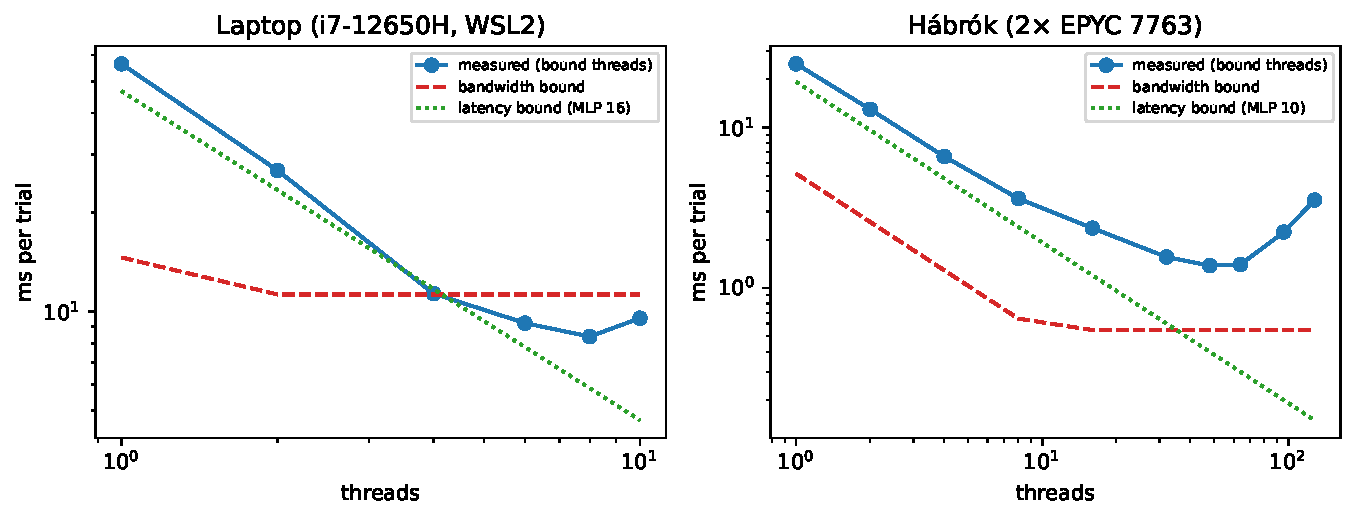
\includegraphics[width=0.9\linewidth]{figures/model.pdf}
\caption{Measured time per search (threads bound) with the bandwidth and latency bounds of
the model.}
\label{fig:model}
\end{figure}

We see three different cases:
\begin{enumerate}
  \item \textbf{One thread: limited by latency.} On both machines $T_\text{lat}$ is larger than
        $T_\text{bw}$, so one core cannot have enough misses open to use the bandwidth. On
        the laptop the measured time is \SI{21}{\percent} above the latency bound. On Hábrók it
        is 2.8 times the bound. This means the BFS only keeps about 7.7 misses open
        ($N_\text{rand} L_\text{DRAM} / T$), while the core could keep 21.7. Every checked
        vertex is a chain of loads that depend on each other (\texttt{parent[u]}, then the
        index, then the neighbour, then the bitmap word), so the out-of-order window only sees
        a few vertices at the same time. On the laptop the latency is much higher, so this
        limit is less visible there. To improve the model, we would have to use the MLP that
        BFS can really reach instead of the maximum of the core.
  \item \textbf{Laptop with all threads: limited by bandwidth.} With 8 threads the latency
        bound is below the bandwidth bound of \SI{11.3}{ms}. The measured \SI{8.4}{ms} is even
        \SI{26}{\percent} faster than this bound. Moving all \SI{179}{MB} from main memory in
        \SI{8.4}{ms} would need \SI{21}{GB/s}, which is more than the \SI{15.9}{GB/s} of
        STREAM, so part of the data comes from the \SI{24}{MiB} L3. \texttt{parent}
        (\SI{4}{MB}), the bitmaps and part of the index fit there. The laptop is at its
        bandwidth limit, which explains why more threads do not help
        (Figure~\ref{fig:scaling}).
  \item \textbf{Hábrók with many threads: neither bound.} Both bounds go down to about
        \SI{0.5}{ms}, but the best measured time is \SI{1.38}{ms} (2.5 times the bound), and
        with 128 threads it is 6.5 times the bound. The missing time is synchronisation
        (about ten barriers per search with up to 128 threads), unbalanced work, and coherence
        traffic between the two sockets. None of these are in a bandwidth and latency model.
        This explains why the Hábrók node is only 3 times faster than the laptop. It also
        shows that on Hábrók we should reduce the number of threads or the synchronisation,
        not the memory traffic.
\end{enumerate}

\paragraph{Attainable performance.} If we write the bound as GTEPS ($m/T_\text{model}$), the
laptop can reach \SI{1.4}{GTEPS} when all data comes from main memory. Because of the L3 we
already reach \SI{1.87}{GTEPS}, so there is not much more to gain without reducing $Q$. On
Hábrók the bound is about \SI{28}{GTEPS} for \texttt{kron20}, and our best result is
\SI{11.4}{GTEPS}. So Hábrók still has room, but only for optimisations that reduce
synchronisation, place the threads and data better, or reduce $Q$ with better locality.

% Owners: 7.1-7.2 Cosmin, 7.3-7.6 Sergiu
\section{Optimisations}
\label{sec:opt}

Each strategy below is motivated by the analysis or the model. Every variant passes the BFS
verifier. Figure~\ref{fig:opt} summarises speed-ups on \texttt{kron20}, and
Table~\ref{tab:opt} gives medians and IQRs. Following Section~\ref{sec:method}, we call a
difference significant only if it exceeds the IQR of both configurations.

\begin{figure}[ht]
\centering
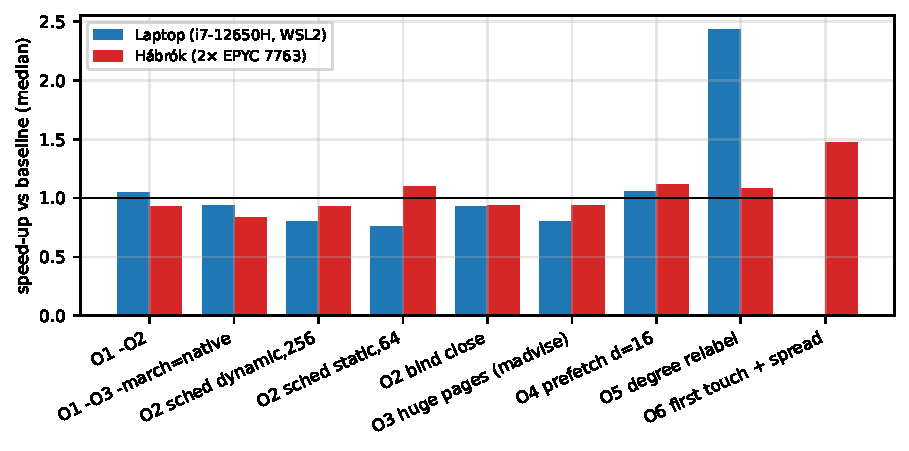
\includegraphics[width=0.9\linewidth]{figures/optimisations.pdf}
\caption{Speed-up of selected variants over the baseline (\texttt{kron20}, all threads,
ratio of medians).}
\label{fig:opt}
\end{figure}

\begin{table}[ht]
\centering\footnotesize
\caption{Median [IQR] in ms per search. Baseline: \texttt{-O3}, default schedule and threads.
Bold: significant improvement.}
\label{tab:opt}
\begin{tabular}{@{}llll@{}}
\toprule
Variant & Graph & Laptop & Hábrók \\
\midrule
Baseline & kron20 & 8.58 [4.77] & 2.85 [1.43] \\
O1 \texttt{-O0} / \texttt{-O2} / \texttt{-O3 -march=native} & kron20 & 20.3 / 8.22 / 9.16 & 7.03 / 3.07 / 3.43 \\
O2 \texttt{static,64} / \texttt{dynamic,256} (both loops) & kron20 & 11.3 / 10.7 & 2.59 [3.21] / 3.08 \\
O2 threads = 8 (laptop) / 48 (Hábrók), bound & kron20 & 8.39 [1.23] & \textbf{1.38 [0.57]} \\
O3 THP \texttt{never} / \texttt{madvise} / patch / \texttt{always} & kron20 & 9.98 / 11.75 / 10.72 / 8.24 & -- / -- / 3.05 / 2.97 \\
O3 huge-page patch & kron22 & 50.2 [43.2] vs.\ 71.1 [58.5] & 12.83 vs.\ 12.14 \\
O4 prefetch $d{=}16$ & kron20 & 8.15 [3.70] & 2.55 [1.57] \\
O5 degree relabelling & kron20 & \textbf{3.53 [1.77]} & 2.64 [3.13] \\
O5 degree relabelling & kron22 & \textbf{25.1 [12.8]} vs.\ 71.1 & \textbf{6.67 [1.35]} vs.\ 12.14 [1.66] \\
O5 degree relabelling & kron24 & -- & 33.7 [17.3] vs.\ 38.2 [5.7] \\
O6 base vs.\ first touch, spread binding & kron20 & -- & 4.00 [1.17] vs.\ \textbf{1.94 [1.18]} \\
O6 base vs.\ first touch, spread binding & kron22 & -- & 12.33 [1.21] vs.\ \textbf{10.96 [1.35]} \\
O7 $\alpha{=}15,\beta{=}9$ / $\alpha{=}5,\beta{=}9$ & kron20 & 8.17 / 37.8 & 2.42 [1.34] / 2.76 \\
\bottomrule
\end{tabular}
\end{table}

\subsection{O1: Compiler optimisation and vectorisation}
\emph{Rationale.} This is the cheapest lever, and it is in our work plan. \emph{Result.}
\texttt{-O0} is 2.4$\times$ slower than \texttt{-O3} on both machines; \texttt{-O1} recovers
most of it; \texttt{-O2} and \texttt{-O3} are indistinguishable within the IQR.
\texttt{-march=native} is not faster (\SI{9.16}{ms} vs.\ \SI{8.01}{ms} on the laptop,
\SI{3.43}{ms} vs.\ \SI{2.75}{ms} on Hábrók, both within the IQR). The GCC vectorisation
report explains why: no hot loop is vectorised. The \texttt{BUStep} inner loop is rejected
because of \emph{control flow in loop} (the early \texttt{break}), its outer loop because of
\emph{multiple nested loops}, and \texttt{TDStep} because the atomic compare-and-swap
\emph{clobbers memory}. Vectorising BFS would need a different algorithm formulation. For
the same reason we did not apply the classic loop transformations (unrolling, unroll-and-jam,
interchange): BFS's loops have data-dependent trip counts and early exits, and
\texttt{-O3} already unrolls where possible. The model also shows the bottleneck is in the
memory system, so the instruction count matters little once \texttt{-O1} has removed the
gross overhead.

\subsection{O2: OpenMP scheduling, binding and thread count}
\emph{Rationale.} Half of the samples are spent in the OpenMP runtime
(Table~\ref{tab:hotspots}), and on Hábrók the model leaves a factor 2.5--6.5 unexplained
(Section~\ref{sec:model}). \emph{Change.} \texttt{schedule(runtime)} for both step loops,
swept over chunk sizes that are multiples of 64 (Section~\ref{sec:method}); thread binding;
thread count. \emph{Result.} No schedule beats the upstream combination (static top-down,
\texttt{dynamic,1024} bottom-up). Applying one schedule to both loops is worse on the laptop,
and Hábrók's best (\texttt{static,64}, \SI{2.59}{ms}) is within the IQR. Binding alone is not
significant. Choosing the thread count is significant: on Hábrók, 48 threads bound to
consecutive cores (\SI{1.38}{ms}) are \textbf{2.1$\times$ faster} than the default 128
unbound threads. They stay on one socket, avoid cross-socket coherence traffic, and pay for
smaller barriers. On the laptop the optimum is 8 of 10 vCPUs, which is not significant.

\subsection{O3: Huge pages}
\emph{Rationale.} The latency curve (Figure~\ref{fig:latency}) rises beyond the TLB reach,
and \texttt{BUStep} and \texttt{TDStep} access a \SI{136}{MB} CSR at random. \emph{Change.}
\texttt{madvise(MADV\_HUGEPAGE)} on the CSR arrays and \texttt{pvector}s before first touch;
we confirmed with \texttt{/proc/self/smaps\_rollup} that \SI{127}{MB} of the process then uses
\SI{2}{MB} pages, against 0 without the patch. \emph{Result.} On \texttt{kron20} all four
laptop configurations lie within each other's IQR. On \texttt{kron22} the patch reduces the
laptop median by \SI{29}{\percent}, but with IQRs above \SI{40}{ms} this is not significant.
Hábrók already runs with THP \texttt{always}, so the baseline uses huge pages and the patch
changes nothing: \num{4200} vs.\ \num{4900} dTLB misses per search, both negligible against
about 2 million random accesses. On the laptop, where TLB misses inflate DRAM latency
(Figure~\ref{fig:latency}), the expected benefit is masked by WSL2's variance.

\subsection{O4: Software prefetching in top-down}
\emph{Rationale.} \texttt{TDStep}'s random \texttt{parent[v]} accesses are latency-bound, and
prefetching $d$ neighbours ahead should increase memory-level parallelism. \emph{Result.}
No distance is significant on either machine (best: $d{=}16$ on Hábrók, $-$\SI{11}{\percent},
within the IQR). The analysis predicts this. Top-down accounts for only \SI{3}{\percent} of the
samples and \SI{11}{\percent} of the modelled traffic, so even perfect prefetching could save
a few per cent (Amdahl's law). The bottom-up step, where the time goes, already issues
independent loads for consecutive vertices, which the out-of-order core overlaps.

\subsection{O5: Degree-ordered relabelling}
\emph{Rationale.} The model says the dominant traffic is one neighbour-list line per vertex
checked in bottom-up, plus random accesses to \texttt{parent}. Renumbering vertices by
decreasing degree (\texttt{-DRELABEL}, using \gapbs' \texttt{RelabelByDegree}) gives the hubs
small, adjacent IDs, which improves locality. Because neighbour lists are sorted, hubs, which
are most likely to be in the frontier, also come first in every list. \emph{Result.} This
is the most effective optimisation: \textbf{2.4$\times$} on the laptop (\texttt{kron20}),
\textbf{2.8$\times$} on the laptop and \textbf{1.8$\times$} on Hábrók for \texttt{kron22}. Our
edge counters show why it works: relabelling reduces the edges examined per search by
\SI{35}{\percent} (\texttt{kron20}) and \SI{48}{\percent} (\texttt{kron22}), because
bottom-up finds a frontier parent sooner. So it reduces both $Q$ and the work. On
\texttt{kron24} the gain is not significant (1.13$\times$, IQR \SI{17}{ms}).
\emph{Caveats.} The one-off relabelling (\SI{0.46}{s} for \texttt{kron20}) is excluded from
the search time and pays off after about 90 laptop searches. Relabelled graphs have different
vertex IDs, so the pseudo-random sources differ from the baseline's.

\begin{figure}[ht]
\centering
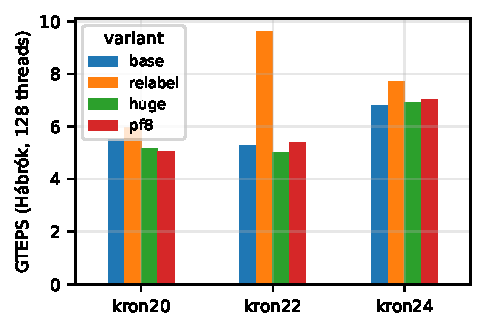
\includegraphics[width=0.48\linewidth]{figures/big_graphs.pdf}
\caption{GTEPS on Hábrók for growing graphs: relabelling helps most on \texttt{kron22}; huge
pages and prefetching do not matter on this node.}
\label{fig:big}
\end{figure}

\subsection{O6: NUMA-aware first touch}
\emph{Rationale.} Loading the graph with a single \texttt{read()} touches every page from one
thread, so on Hábrók the whole \SI{125}{MB} edge array lands on one socket. The second
socket's threads then read everything remotely, and only one socket's memory controllers are
used. \texttt{numactl} is not available, so \emph{change}: \texttt{-DPAR\_FIRST\_TOUCH}
zeroes the array in parallel before reading. \emph{Result.} Placement matters as soon as
threads are spread over both sockets. With \texttt{OMP\_PROC\_BIND=spread}, the baseline
slows to \SI{4.00}{ms} [IQR 1.17] on \texttt{kron20}, because half of the threads read
everything remotely. With parallel first touch it takes \textbf{\SI{1.94}{ms} [1.18], a
2.1$\times$ improvement}, and 1.5$\times$ faster than the default configuration. On
\texttt{kron22} first touch gains \SI{11}{\percent} with spread binding (\SI{12.33}{} $\to$
\SI{10.96}{ms}, significant). Unbound, the gains are smaller and within the IQR, because the
OS places threads unpredictably. On \texttt{kron24} the difference is not significant; we have
not yet determined why the effect disappears for the largest graph.

\subsection{O7: Direction-switch thresholds}
\emph{Rationale.} $\alpha$ and $\beta$ decide how much work runs in the two very different
steps. \emph{Result.} A $3\times3$ sweep shows the defaults are near-optimal. $\alpha{=}5$
keeps the search top-down for too long and is 4.4$\times$ slower on the laptop. The best
settings ($\alpha{=}15,\beta{=}36$ on the laptop, $\alpha{=}15,\beta{=}9$ on Hábrók) are
within the IQR of the defaults.

% Owners: both
\section{Discussion and conclusion}
\label{sec:conclusion}

\paragraph{What limits BFS.} Combining profiles, edge counts and the model gives a
consistent picture. A single core is latency-bound: it cannot keep enough misses in flight.
A laptop with all cores is bandwidth-bound and already beyond its DRAM bound thanks to L3
reuse. A 128-core server is bound by neither: synchronisation at about ten barriers per
search and cross-socket effects dominate. The optimisations confirm this. The significant ones reduce memory traffic or work
(relabelling), synchronisation span (fewer, socket-local threads), or remote memory traffic
(NUMA-aware first touch). Those that target instruction count (compiler flags, vectorisation) or a
minor kernel (prefetching in top-down) were not. This matches the course's message: the
justification from analysis and model predicted which strategies could pay off before they
were implemented.

\paragraph{Threats to validity.}
(i)~The laptop ran under WSL2: no hardware counters, a hidden hybrid topology and high
variance (IQR up to \SI{56}{\percent}). We therefore use medians and treat differences within
the IQR as insignificant. (ii)~The model assumes every byte comes from DRAM; this is why the
laptop beats its bound. A cache-aware refinement would use the L3 bandwidth for the
\SI{4}{MB} \texttt{parent} array. (iii)~Hábrók's counters were multiplexed, and the 128-thread counter runs include warm-up
trials, so we use only single-thread counters quantitatively.
(iv)~Relabelling changes the source vertices. (v)~\texttt{kron20} is small for a 128-core
node. Results on \texttt{kron22}/\texttt{kron24} show the expected higher GTEPS with
growing work per barrier (\SI{6.8}{GTEPS} on \texttt{kron24}).

\paragraph{Future work.} Hardware counters on the laptop through a native Linux boot, which
would also allow a top-down microarchitecture analysis; the Apple Silicon comparison planned
in our work plan; a branch-free bitmap test in \texttt{BUStep} against the
\SI{12.9}{\percent} misprediction rate; a NUMA-aware partitioning of the bottom-up sweep; and
fusing the short parallel regions of a BFS level to remove barriers, analogous to loop
fusion. The last one addresses the dominant cost we identified.


\section{Workload distribution}
\begin{center}
\begin{tabular}{|l|l|}
\hline
Name & Parts \\
\hline
Cosmin Andrei Stamate & laptop measurements, Sections 3, 4, 5, 7.1, 7.2 \\
Sergiu Alexandru Macra & Hábrók measurements, Sections 1, 2, 6, 7.3 to 7.7 \\
Both & scripts, analysis, Section 8 \\
\hline
\end{tabular}
\captionof{table}{Workload}
\end{center}

\begin{thebibliography}{9}
\bibitem{beamer2015gap} S.~Beamer, K.~Asanović, D.~Patterson. \emph{The GAP Benchmark Suite}. arXiv:1508.03619, 2015.
\bibitem{beamer2012do} S.~Beamer, K.~Asanović, D.~Patterson. \emph{Direction-Optimizing Breadth-First Search}. SC'12, 2012.
\bibitem{mccalpin} J.~D.~McCalpin. \emph{STREAM: Sustainable Memory Bandwidth in High Performance Computers}. \url{https://www.cs.virginia.edu/stream/}.
\bibitem{roofline} S.~Williams, A.~Waterman, D.~Patterson. \emph{Roofline: an insightful visual performance model for multicore architectures}. CACM 52(4), 2009.
\bibitem{papi} PAPI: Performance Application Programming Interface, ICL, University of Tennessee. \url{https://icl.utk.edu/papi/}.
\bibitem{graph500} Graph500 Benchmark Specification. \url{https://graph500.org}.
\end{thebibliography}

\appendix
\section*{Code and data}
All code, scripts and raw results are in \url{https://github.com/CosminStamateAndrei/gapbs}
(folder \texttt{pe/}). The file \texttt{pe/README.md} explains how to reproduce every result.
\end{document}
